% Drawing 121/02-1 -- folder 121, batch 02, archive page 40 (PDF page 41).
% Transcription: Croquis : à gauche, les trois $V_0^\circ$, $V_1^\circ$, $V_2^\circ$, avec $\partial V_1^\circ \to V_0^\circ$ et $\partial V_2^\circ = \partial_1 V_2^\circ \cup \partial_0 V_2^\circ$ envoyé sur $V_1^\circ$ et $V_0^\circ$ par des flèches courbes ; en bas, un tableau de flèches $\partial_2 \leftarrow \partial_{21}$, $\partial_{20} \leftarrow \partial_{210}$, $\partial_1 \leftarrow \partial_{10}$, $\partial_0 \leftarrow \ldots$, avec « bord » ; deux bandes hachurées étiquetées $\partial_{210}$, $\partial_{20}$, $\partial_{21}$ ; un cylindre et un tore étiquetés $\partial_{10}$, $\partial_1$ ; un grand cercle $\partial_0$ contenant une haltère $\partial_0$ ; dans un cadre, $\partial_1$, $\partial_{10}$, $\partial_0 = \partial_0$, et un demi-cercle posé sur un segment, marqué $\partial_1\ \partial_0\ \partial_1$
% Kind: page of sketches: V_i^o with boundary maps, table of boundary arrows, bands, cylinder, circle with dumbbell, framed figure. Method 2 (schematic redraw from the facsimile). Status: partial.
% Notes: Lower half of the sheet (the formulas above are text). The scheme V_0^o, V_1^o, V_2^o with the arrows from their boundaries; the table of arrows d_2 <- d_21, d_20 <- d_210, d_1 <- d_10, d_0 <- ... with "bord" and curved arrows (schematised); two hatched bands with their labels; a cylinder and a torus-like tube labelled d_10, d_1; a large circle d_0 containing a dumbbell d_0; in a frame d_1, d_10, d_0 = d_0 and a half-circle on a segment marked d_1 d_0 d_1. Small labels are placed after the transcription; the curved arrows of the table and some small labels inside the tube are approximate. The name written at the top of the sheet (Fujii Guruji Nichidatsu, a public religious figure) is not part of the mark.
% Coordinates: 1 unit = 1 mm = 1/100 of the crop width (bbox in page fractions: [0.04, 0.04, 0.97, 0.88]).
% Redrawn by Claude (claude-opus-5-5), issue #73, 2026-11-07; not checked by a human; not compiled (no TeX in the session).
% Rights: reproduces part of the work -- behind RENDER_TRANSCRIPTS, never published by itself.
\documentclass[tikz,border=3pt]{standalone}
\usepackage{amsmath,amssymb}
\usetikzlibrary{patterns,arrows.meta}
\tikzset{pencil/.style={black!45}, struck/.style={black!35}, mark/.style={circle,draw,inner sep=1.3pt}, pt/.style={circle,fill,inner sep=0.9pt}, opt/.style={circle,draw,fill=white,inner sep=1.1pt}}
\begin{document}
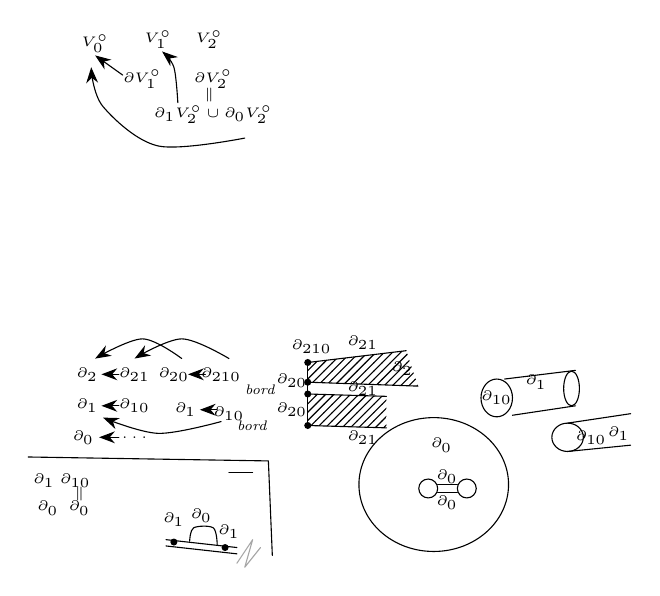
\begin{tikzpicture}[x=1mm,y=1mm,line cap=round,line join=round,font=\scriptsize]
\node[inner sep=1pt] at (22,-59) {\tiny $V_0^\circ$};
\node[inner sep=1pt] at (30,-58.5) {\tiny $V_1^\circ$};
\node[inner sep=1pt] at (36.5,-58.5) {\tiny $V_2^\circ$};
\node[inner sep=1pt] at (28,-63.5) {\tiny $\partial V_1^\circ$};
\draw[-{Stealth[length=2mm]}] (25.5,-63) -- (22,-60.5);
\draw[-{Stealth[length=2mm]}] plot[smooth, tension=0.55] coordinates {(32.5,-66.5) (32,-62) (30.5,-60)};
\node[inner sep=1pt] at (37,-63.5) {\tiny $\partial V_2^\circ$};
\node[inner sep=1pt] at (36.5,-65.5) {\tiny $\parallel$};
\node[inner sep=1pt] at (37,-68) {\tiny $\partial_1V_2^\circ\cup\partial_0V_2^\circ$};
\draw[-{Stealth[length=2mm]}] plot[smooth, tension=0.55] coordinates {(41,-71) (30,-72) (23,-67) (21.5,-62)};
\node[inner sep=1pt] at (21,-101) {\tiny $\partial_2$};
\node[inner sep=1pt] at (27,-101) {\tiny $\partial_{21}$};
\node[inner sep=1pt] at (32,-101) {\tiny $\partial_{20}$};
\node[inner sep=1pt] at (38,-101) {\tiny $\partial_{210}$};
\draw[-{Stealth[length=2mm]}] (25,-101) -- (22.8,-101);
\draw[-{Stealth[length=2mm]}] (36,-101) -- (33.8,-101);
\node[inner sep=1pt] at (21,-105) {\tiny $\partial_1$};
\node[inner sep=1pt] at (27,-105) {\tiny $\partial_{10}$};
\draw[-{Stealth[length=2mm]}] (25,-105) -- (22.8,-105);
\node[inner sep=1pt] at (33.5,-105.5) {\tiny $\partial_{1}$};
\node[inner sep=1pt] at (39,-106) {\tiny $\partial_{10}$};
\draw[-{Stealth[length=2mm]}] (37.5,-105.5) -- (35.3,-105.5);
\node[inner sep=1pt] at (20.5,-109) {\tiny $\partial_0$};
\draw[-{Stealth[length=2mm]}] (25,-109) -- (22.5,-109);
\node[inner sep=1pt] at (27,-109) {\tiny $\ldots$};
\node[inner sep=1pt] at (43,-103) {\tiny \textit{bord}};
\node[inner sep=1pt] at (42,-107.5) {\tiny \textit{bord}};
\draw[-{Stealth[length=2mm]}] plot[smooth, tension=0.55] coordinates {(33,-99) (28,-96.5) (22,-99)};
\draw[-{Stealth[length=2mm]}] plot[smooth, tension=0.55] coordinates {(39,-99) (33,-96.5) (27,-99)};
\draw[-{Stealth[length=2mm]}] plot[smooth, tension=0.55] coordinates {(38,-107) (30,-108.5) (23,-106.5)};
\draw (49,-99.5) -- (61.5,-98);
\draw (49,-102) -- (63,-102.5);
\fill[pattern=north east lines] (49,-99.5) -- (61.5,-98) -- (63,-102.5) -- (49,-102) -- cycle;
\draw (49,-103.5) -- (59,-103.8);
\draw (49,-107.5) -- (59,-107.8);
\fill[pattern=north east lines] (49,-103.5) -- (59,-103.8) -- (59,-107.8) -- (49,-107.5) -- cycle;
\draw (49,-99.5) -- (49,-107.5);
\node[pt] at (49,-99.5) {};
\node[pt] at (49,-102) {};
\node[pt] at (49,-103.5) {};
\node[pt] at (49,-107.5) {};
\node[inner sep=1pt] at (49.5,-97.5) {\tiny $\partial_{210}$};
\node[inner sep=1pt] at (56,-97) {\tiny $\partial_{21}$};
\node[inner sep=1pt] at (61,-100.3) {\tiny $\partial_2$};
\node[inner sep=1pt] at (47,-101.8) {\tiny $\partial_{20}$};
\node[inner sep=1pt] at (56,-102.8) {\tiny $\partial_{21}$};
\node[inner sep=1pt] at (47,-105.5) {\tiny $\partial_{20}$};
\node[inner sep=1pt] at (56,-109) {\tiny $\partial_{21}$};
\draw (73,-104) ellipse[x radius=2, y radius=2.4];
\node[inner sep=1pt] at (73,-104) {\tiny $\partial_{10}$};
\draw (74,-101.6) -- (83,-100.5);
\draw (75,-106.2) -- (83,-105);
\draw (82.5,-102.8) ellipse[x radius=1, y radius=2.2];
\node[inner sep=1pt] at (78,-102) {\tiny $\partial_1$};
\draw (82,-109) ellipse[x radius=2, y radius=1.8];
\draw (82,-107.2) -- (90,-106);
\draw (82,-110.8) -- (90,-110);
\node[inner sep=1pt] at (85,-109) {\tiny $\partial_{10}$};
\node[inner sep=1pt] at (88.5,-108.5) {\tiny $\partial_1$};
\draw (65,-115) ellipse[x radius=9.5, y radius=8.5];
\node[inner sep=1pt] at (66,-110) {\tiny $\partial_0$};
\draw (64.3,-115.5) circle[radius=1.2];
\draw (69.2,-115.5) circle[radius=1.2];
\draw (65.5,-115) -- (68,-115);
\draw (65.5,-116) -- (68,-116);
\node[inner sep=1pt] at (66.7,-114) {\tiny $\partial_0$};
\node[inner sep=1pt] at (66.7,-117.3) {\tiny $\partial_0$};
\draw (13.5,-111.5) -- (44,-112) -- (44.5,-124);
\draw (39,-113.5) -- (42,-113.5);
\node[inner sep=1pt] at (15.5,-114.5) {\tiny $\partial_1$};
\node[inner sep=1pt] at (19.5,-114.5) {\tiny $\partial_{10}$};
\node[inner sep=1pt] at (20,-116.2) {\tiny $\parallel$};
\node[inner sep=1pt] at (16,-118) {\tiny $\partial_0$};
\node[inner sep=1pt] at (20,-118) {\tiny $\partial_0$};
\draw (31,-122) -- (40,-123);
\draw (31,-122.8) -- (40,-123.8);
\draw plot[smooth, tension=0.55] coordinates {(34,-122.2) (34.5,-120.5) (37,-120.5) (37.5,-122.6)};
\node[pt] at (32,-122.3) {};
\node[pt] at (38.5,-123) {};
\node[inner sep=1pt] at (32,-119.5) {\tiny $\partial_1$};
\node[inner sep=1pt] at (35.5,-119) {\tiny $\partial_0$};
\node[inner sep=1pt] at (39,-121) {\tiny $\partial_1$};
\draw[struck] (40,-125) -- (42,-122) -- (41,-125.5) -- (43,-123);
\end{tikzpicture}
\end{document}
